%
% stm-java.tex
% @author Sidharth Mishra
% @description Information about STM in java
% @copyright 2017 Sidharth Mishra
% @created Thu Dec 07 2017 19:08:54 GMT-0800 (PST)
% @last-modified Thu Dec 07 2017 19:08:54 GMT-0800 (PST)
%

\documentclass[../main]{subfiles}
  
\begin{document}

  \section{STM in Java}

  \par
  This section discusses the implementation of the STM prototype in {\em Java}. Figure \ref{fig:stm-java} is the UML class diagram of the STM prototype implemented in {\em Java}.

  \begin{figure}[h]
    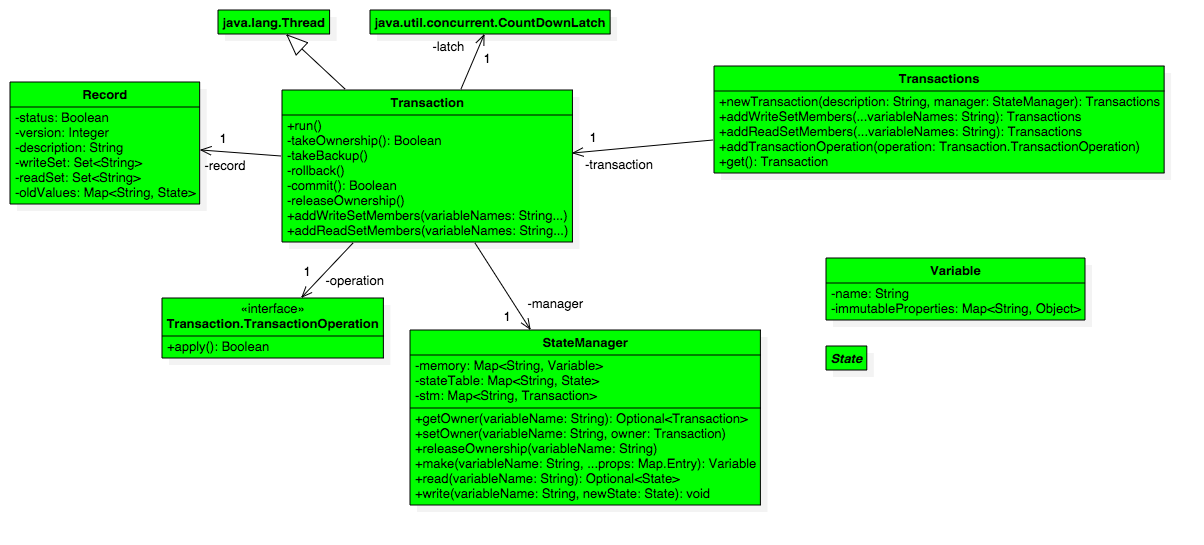
\includegraphics[width=\textwidth]{stm-java.png}
    \caption{UML for STM prototype in {\em Java}}
    \label{fig:stm-java}
  \end{figure}

  \par
  In this prototype, the \code{StateManager} is the shared object/memory --- the STM. It has a field called \code{memory} which is a {\em hash-map} mapping a \code{String} to \code{Variable}. In this prototype, I was influenced by {\em Haskell}'s {\em Map} and tried to break the data into two parts --- mutable and immutable. The immutable part is the identifying information and is held inside the \code{Variable} object. The mutable part is held inside \code{State} --- \code{State} is an abstract class that the consumer of the library needs to extend to make their data storable inside the memory cells. The \code{stateTable} associates both the mutable and immutable parts of the data --- the \code{stateTable} is a {\em hash-map} from \code{String} to \code{State}. The \code{stateTable} and the \code{memory} together represent the {\em Memory} of the STM. \par

  The \code{stm} in the \code{StateManager} is the {\em Ownerships} and it is a {\em hash-map} instead of a {\em Vector}. The \code{stm} --- {\em Ownerships} --- maps from \code{String} to \code{Transaction}. I use strings instead of memory addresses in {\em Java}. \par 
  
  The \code{StateManager} provides the APIs to set the owner of a memory cell (\code{setOwner}), get the owner of a memory cell (\code{getOwner}), release the memory cell from the ownership of a transaction (\code{releaseOwnership}), read data from a memory cell (\code{read}), write data into a memory cell (\code{write}), and make a memory cell (\code{make}). \par

  Also, I use {\em Project Lombok} to get annotation processors to reduce boilerplate code. The class \code{Record} is used to hold the metadata of a \code{Transaction}. \code{Record} contains the \code{readSet}, \code{writeSet}, and \code{oldValues}. The \code{readSet}, \code{writeSet} are used to hold the names (addresses) of the memory cells that the \code{Transaction} intends to read-from and write-to respectively. The \code{oldValues} is a {\em hash-map} from memory cell name/address to the data it contains and works as the backup which needs to be restored incase the transaction fails / aborts. \par

  The \code{Transaction} represents the thread of control. It extends from \code{java.lang.Thread} class. It follows the execution workflow defined in the Section \ref{sec:exec-workflow}. \code{TransactionOperation} is a static \code{FunctionalInterface} defined inside the \code{Transaction} class which represents the action that the transaction needs to do. \par

  The \code{Transactions} utility is used for creating transactions. Following is an example displaying the usage of the APIs. The full source code of the example can be found in the \code{foop.test.bank.BankDriver} class. I use {\em JUnit} to write test cases/examples usages for this prototype and {\em SLF4J-Logback} for logging. The example used in this test is a simple bank transaction simulation, it has two methods \code{deposit} and \code{withdraw}. \par

  The \code{deposit} and \code{withdraw} methods are defined as: \par

  \begin{lstlisting}

    /**
    * <p>
    * A probable method for taking care of bank account operations
    * Deposits the amount into the bank account
    * 
    * @param account
    *            The bank account name
    * @param amount
    *            The amount to be deposited
    */
    private static void deposit(String account, float amount) {
      logger.info(
        String.format("Depositing amount:: %f into bank account:: %s", 
          amount, account));
    
      // read data from the memory cell named by the account name
      AccountBalance b = manager.read(account).isPresent() 
        ? (AccountBalance) manager.read(account).get()
        : new AccountBalance(0);
    
      AccountBalance bnew = new AccountBalance(b.getBalance() + amount);
    
      // write data into the memory cell, that is the new amount
      // in the account.
      manager.write(account, bnew);
    
      logger.info(
        String.format(
          "Deposited amount:: %f into bank account:: %s, new amount:: %f", 
          amount, account,
          ((AccountBalance) manager.read(account).get()).getBalance()));
    }

  /**
  * <p>
  * Another probable method for taking care of bank account operations
  * Withdraws the specified amount from bank accounts
  * 
  * @param account
  *            The bank account name
  * 
  * @param amount
  *            The amount of money to be withdrawn
  */
  private static void withdraw(String account, float amount) {
       
      logger.info(
        String.format("Withdrawing amount:: %f into bank account:: %s", 
          amount, account));
      
      // reading data from the memory cell
      AccountBalance b = manager.read(account).isPresent() 
        ? (AccountBalance) manager.read(account).get()
        : new AccountBalance(0);
       
      AccountBalance bnew = new AccountBalance(b.getBalance() - amount);
      
      // writing data into the memory cell
      manager.write(account, bnew);
       
      logger.info(
        String.format("Withdrew amount:: %f into bank account:: %s, new amount:: %f", 
          amount, account,
          ((AccountBalance) manager.read(account).get()).getBalance()));
  }
  \end{lstlisting}

  Since, \code{AccountBalance} is the data being stored in the memory cells, it must comply with the \code{State} and \code{Variable} format that the memory cell dictates its contents to be. So, \code{AccountBalance} looks like: \par

  \begin{lstlisting}
    /**
    * @author sidmishraw
    *
    *     Qualified Name: foop.test.bank.AccountBalance
    *
    */
    @EqualsAndHashCode(callSuper = false)
    @ToString
    public class AccountBalance extends State {

      private @Getter float balance;

      /**
      * @param balance
      */
      public AccountBalance(float balance) {
        this.balance = balance;
      }
    }
  \end{lstlisting}

  The \code{@ToString}, \code{@EqualsAndHashCode}, and \code{@Getter} are annotations provided by {\em Project Lombok} and they auto-generate the methods they are named after --- boilerplate reduction. \par

  Following are excerpts from the \code{BankDriver} class. This class displays the API usage. 
  
  \begin{lstlisting}

    // manager is the singleton instance of the
    // StateManager class --- the STM
    private static StateManager manager = InstanceFactory.getInstance(StateManager.class);

    // ts is the singleton instance of the Transactions utility 
    // for creating transactions.
    private static Transactions ts = InstanceFactory.getInstance(Transactions.class);


    ...

    // make memory cells to hold data
    // in this case, bank accounts
    manager.make("Account1");

    ...

    // t is a transaction object constructed using the Transactions 
    // utility. The Transactions utility only supports adding one
    // operation but, the operation is a ``lambda''
    Transaction t = ts.newTransaction("T1", manager)
        .addWriteSetMembers("Account1", "Account2")
        .addReadSetMembers("Account1", "Account2")
        .addTransactionOperation(() -> {
            
            withdraw("Account2", 500.00F);
            deposit("Account1", 500.00F);
            
            return true;
        })
        .get();
    
    t.setName("T1"); // sets the name of the transaction object
    
    t.setLatch(new CountDownLatch(1));  // sets the CountDownLatch
                                        // for the transaction so 
                                        // that the calling thread can
                                        // wait till the transaction
                                        // is done executing 
                                        // --- synchronous execution
    
    t.start(); // starts executing the transaction
    
    try {
        
        // wait on the transaction to complete
        t.join();
    } catch (InterruptedException e) {
        
        logger.error(e.getMessage(), e);
    }

    ...

  \end{lstlisting}

  \par
  \begin{verse}
    Note: The STM prototype in {\em Java} was included in the {\bf Milestone\#1} of the project. The testcases can be found inside the \code{foop.test} package.
  \end{verse}

\end{document}